\documentclass[11pt]{article}
\usepackage[utf8]{inputenc}
\pagestyle{headings}
\usepackage[top=1in, bottom=1in]{geometry}
\usepackage{amsmath,amsfonts,amsthm,amssymb}
\usepackage[pdftex]{graphicx}
\usepackage{url}
\usepackage{subfig}
\usepackage{color}
\usepackage{algorithm}
\usepackage{algorithmic}
\usepackage{amssymb}
\usepackage{ifthen}
\usepackage[pagebackref=true,breaklinks=true,colorlinks,bookmarks=false,citecolor=red,linkcolor=red]{hyperref}

\renewcommand{\algorithmicrequire}{\textbf{Input:}}
\renewcommand{\algorithmicensure}{\textbf{Output:}}

%% Command definitions
\def\subsectionautorefname{section}
\newcommand{\todo}[1]{\textcolor{red}{#1}}
\definecolor{light-gray}{gray}{0.3}
\newcommand{\aside}[1]{\textcolor{light-gray}{\emph{#1}}}
\newcommand{\comment}[1]{}

\newcommand{\shownotes}{0}
\ifthenelse{ \shownotes = 1}
{ \newcommand{\note}[3]{\marginpar{\textcolor{black}{#1:} \textcolor{red}{\emph{#2}}} \textcolor{red}{#3}} }
{ \newcommand{\note}[3]{\textcolor{black}{#3}} }

\title{Recommending Couches to Surf: Machine Learning for Social Travel}
\author{Ron Sun, Tobi Baumgartner, Tim Althoff, Sergey Karayev}
\date{\today}

\begin{document}
\maketitle

\begin{abstract}
New technologies have made social interactions that were previously unthinkable commonplace.
When traveling, a viable new option is to be hosted by a friendly resident of the destination, for free---to ``couchsurf.''
When arranging such accomodation through a web interface, travelers face a daunting list of potential hosts, while hosts in popular destinations are inundated with requests for lodging.
We postulate that some connections are more likely to happen than others, based on general desired compatibility between host and visitor and on personal host preferences.
We present a system for predicting successful host-visitor matches, trained and evaluated on data from the most popular website for this purpose: \url{couchsurfing.com}.
A re-ranking of visitor requests based on our system would be beneficial to the user experience on the website, as hosts would have to look through fewer requests and visitors would be more likely to be matched to a host that is likely to accept them.
\end{abstract}

% !TEX root=report.tex
\section{Introduction}

\begin{quotation}
Among those to whom I did not write “couch requests” were “a travelling magician and professional fool” from New Mexico; a sixty-three-year-old gay semi-retired handyman in Pahoa, Hawaii, whose mission is “looking for more nudists” (there are plenty of “clothing optional” possibilities on CouchSurfing); another Hawaiian, this one describing himself as “just a guy who has three acres of land, living in a shipping container house”; a woman in Bozeman, Montana, who declared that her “home is oppression-free. Yay!” and also contains high-speed Wi-Fi; a thirty-one-year-old female “daydreamer” from Berkeley who loves pajamas; a Tarot-card reader in Marfa, Texas; a housewife in Charleston, South Carolina, who owns a pole-dancing studio called Dolphin Dance; a kite-surfing physician (again, Charleston) whose ambition is to start a flavored-envelope company; a freelance photographer in San Francisco who claims she’s had hiccups every day for the past five years; a Savannah, Georgia, scientist who is also a “free man,” doing “whatever I want, whenever I want”; a male in Antarctica who wishes to live as a female; a “lovetarian” who grew up in Doylestown, Pennsylvania; ... and eighty-four people in Brunei Darussalam.

-- Patricia Marx. \emph{You're Welcome: Couch-surfing the globe}. New Yorker, April 16, 2012.\footnote{Retrieved from \url{http://www.newyorker.com/reporting/2012/04/16/120416fa_fact_marx}}
\end{quotation}

Our new global interconnectedness has made social interactions that were previously unthinkable commonplace.
Whereas even a few decades ago a traveler had to either have a friend or pay for a hotel for lodging while traveling, today people so inclined can stay for free at complete strangers' residences, in locations that span all countries and continents.
Such accomodations are arranged via special-purpose websites that let users willing to host travelers to list their apartments (``hosts''), and users wanting to with someone for free to request lodging from the hosts (``surfers'').
Among these websites, by far the biggest is CouchSurfing (\url{http://couchsurfing.org/}), a website launched in 2004 now boasting almost four million users.

There is a staggering variety of people on CouchSurfing.
There are members in every country, speaking over three hundred different languages.
The age distribution skews young: the average age is twenty-eight and a third are between 18 and 24.
The website has facilitated over six million positively-reviewed visits, with ``only a tiny fraction of one per cent negative.''\footnote{from the article quoted in the epigraph.}

A fraternizing spirit is strong with most users of the site, as they are willing to host or guest with strangers in exchange for no money.
All the same, we believe that people enjoy the company of kindred spirits the most---or at the least, that there are some user-match relationships that are more successful than others.

\begin{figure}[ht]
\centering

\includegraphics[width=1\linewidth]{figures/screenshots/requests.png}
\caption{Example of a host's inbox view.}
\label{fig:sample_request}
\end{figure}

When a surfer is looking for lodging, they do a search for available couches (or beds, or the floor, as the case may be) in the destination location.
Usually, they are presented with an array of choices, often more than can quickly be looked through---or messaged.
An example of a host's inbox is presented in \autoref{fig:sample_request}.
It would be beneficial to a searching surfer to have hosts that are available, agreeable, and likely to respond positively displayed at the top of the list.
Similarly, hosts in popular locations are inundated with requests for accomodation.
To save time, surfers that would be agreeable to them should be displayed at the top.

Our aim is to facilitate matching surfers and hosts to maximize the acceptance rate of couchrequests. This benefits both surfer and hosts: the surfer has to write less requests in order to find a place to stay, and the host has to review less requests to find a surfer he would like to host.

In private discussion with the CEO and CTO of CouchSurfing, we established that they perceived the second scenario (from the perspective of the hosts) to be prevalent as a negative user experience and more in need of a recommendation system solution than the first (from the perspective of the surfers).

In this work, we develop a system to automatically evaluate the couch requests that hosts get with respect to the likelihood of a successful and pleasant visit, and so make the CouchSurfing experience as convenient as possible.
While we train and evaluate our approach from the perspective of the hosts, our solution to the problem---predicting the probability of a host accepting a surfer request---benefits surfers just as much, as their search results can be ranked according to the likelihood of acceptance to save them message-writing effort.

% !TEX root=report.tex
\subsection{Related Work} \label{sec:related_work}
CouchSurfing data has been used in research in the field of trust and reputation systems \cite{Lauterbach2009}.
Trust and reputation are critical factors for users to decide whom to interact with.
Reputation systems allow users to judge other user's trustworthiness and provides incentives for users to be honest.
For this purpose, CouchSurfing.org employs a vouching system (declaring friends as trustworthy), a verification system (paying a small fee to get your name and address verified---the only revenue source for the website), and references (ratings and feedback) from other users.
In this work, we do not focus on reputation and trust, but rather on other features of surfers and hosts that may signal likelihood of an accepted request.

Recommender systems rely heavily on ratings contributed by users in order to predict other users preferences.
Follow-up work has shown that public, identified ratings tend to be disproportionally positive if the ratee is another user who can reciprocate \cite{Teng2010} (like on CouchSurfing). 
To the best of our knowledge this paper represents the first effort in using recommender systems and machine learning for social travel on platforms like CouchSurfing.
While we make use of ratings as a source of features for our prediction task, predicting the ratings themselves is not our goal.
Rather, we aim to predict which couch request, among a group of competing ones, will be accepted by the host.

A similar problem arises in search engine optimization in a seminal paper on ranking SVMs \cite{Joachims2002}.
Clickthrough data from users presented with a ranked list of results was used to improve the ranking function in a max-margin formulation.
In our situation, hosts are indeed presented with a ranked list of surfers (and surfers with a list of hosts), but the time of presentation as well as the clickthrough data is unknown to us.
We can, however, infer rough presentation times from the request and decision times, and we have the resulting accept or reject decision of the host.
In this way, our problem is of classification and not ranking: given a set of couch requests, we predict, for each one, whether it was accepted or rejected, with the constraint that only one request could have been accepted.

There are two parts to this prediction: a global ``attraction'' model that explains in general why some hosts prefer some users to others; and a host-specific personal model that allows additional flexibility.
Personalizing classifiers in this way leads to a very large number of parameters that often is infeasible to keep in memory.
To enable for personalization in a large-scale setting, the hashing trick has been proposed where either features or parameters are hashed into an array of predefined size.
This potentially allows features or parameters to collide, but it has been successfully applied in personalized spam classification \cite{Attenberg2009} and investigated theoretically \cite{Weinberger2012}.
We use the hashing trick to store personalized host parameters.

Another related strand of research is in predicting friendship connections, which is considered in \cite{Yang2011} using joint information in existing friendships and common interests based on the hypothesis of homophily.
The hypothesis is that people with similar interests attract each other: a premise that our model has sufficient power to express, but is not biased toward.
Similarly, we use the interests of hosts and surfers expressed in free form text on their personal profiles to estimate the likelihood of an accepted request.
Some evaluation schemes in \cite{Yang2011} are also relevant to our problem formulation.

For learning, we use a parallel Stochastic Gradient Descent (SGD) algorithm that distributes random subsets of the data onto multiple machines and uses fast lock-free updates on a local copy of the parameters \cite{Zinkevich2010}.
We modify the algorithm in that after a certain number of iterations, the results are averaged and re-broadcast, for additional robustness.

As part of our featurization function, we extract ``interests'' from free-form text of the user profiles.
In this challenging task we are guided by \cite{Liu2005}, who use a graph structure assembled from overlapping user interests, and \cite{Cantador2011}, who deal with semantic annotation: essentially mapping a document to its ontology entities (almost like topic modeling).
We learn the graph based on a novel normalization scheme, and use clusters found in the structure as features in our model.
\todo{To Ron: update this part of related work as you see fit.}

\comment{They \cite{Cantador2011} extract terms, map the terms to ontology entities (by looking up the term's wikipedia article and construct a vector of applicable ontology entities based on what categories appear in the wikipedia article), and then measure the strength of those mappings using the tf-idf measure.
They build a news recommender system that recommends based on activation propagation.}

\comment{\paragraph{CoFiRank} \cite{Weimer2009}
This paper learns features/latent factors but does not allow for additional observations (apart from ratings).
We, however, have more features we want to use (i.e. demographic and geographic papers).
hey learn how to rank as opposed to how to score and also provide a definition of nDCG.
It leads to a structured estimation SVM-like optimization problem and there seems to be C++ software available.
Still, we should start with an easier (probably linear) model and we might use a classification instead of a ranking framework.}
% !TEX root=report.tex
\section{Data Exploration}

The CouchSurfing dataset was made privately available to the authors in the form of an anonymized MySQL database dump.
In the process of   

\subsection{Host and suitor distribution}
\todo{add visualizations such as the ones Tobi made}

\subsection{Matters of time}
\todo{visualize and discuss the kind of plots we've been drawing on the white board showing viability and preference order of requests}

\subsection{User interests}
% !TEX root=report.tex
\section{Problem Formalization and Prediction Model} \label{sec:model}

\begin{figure}[ht]
\centering
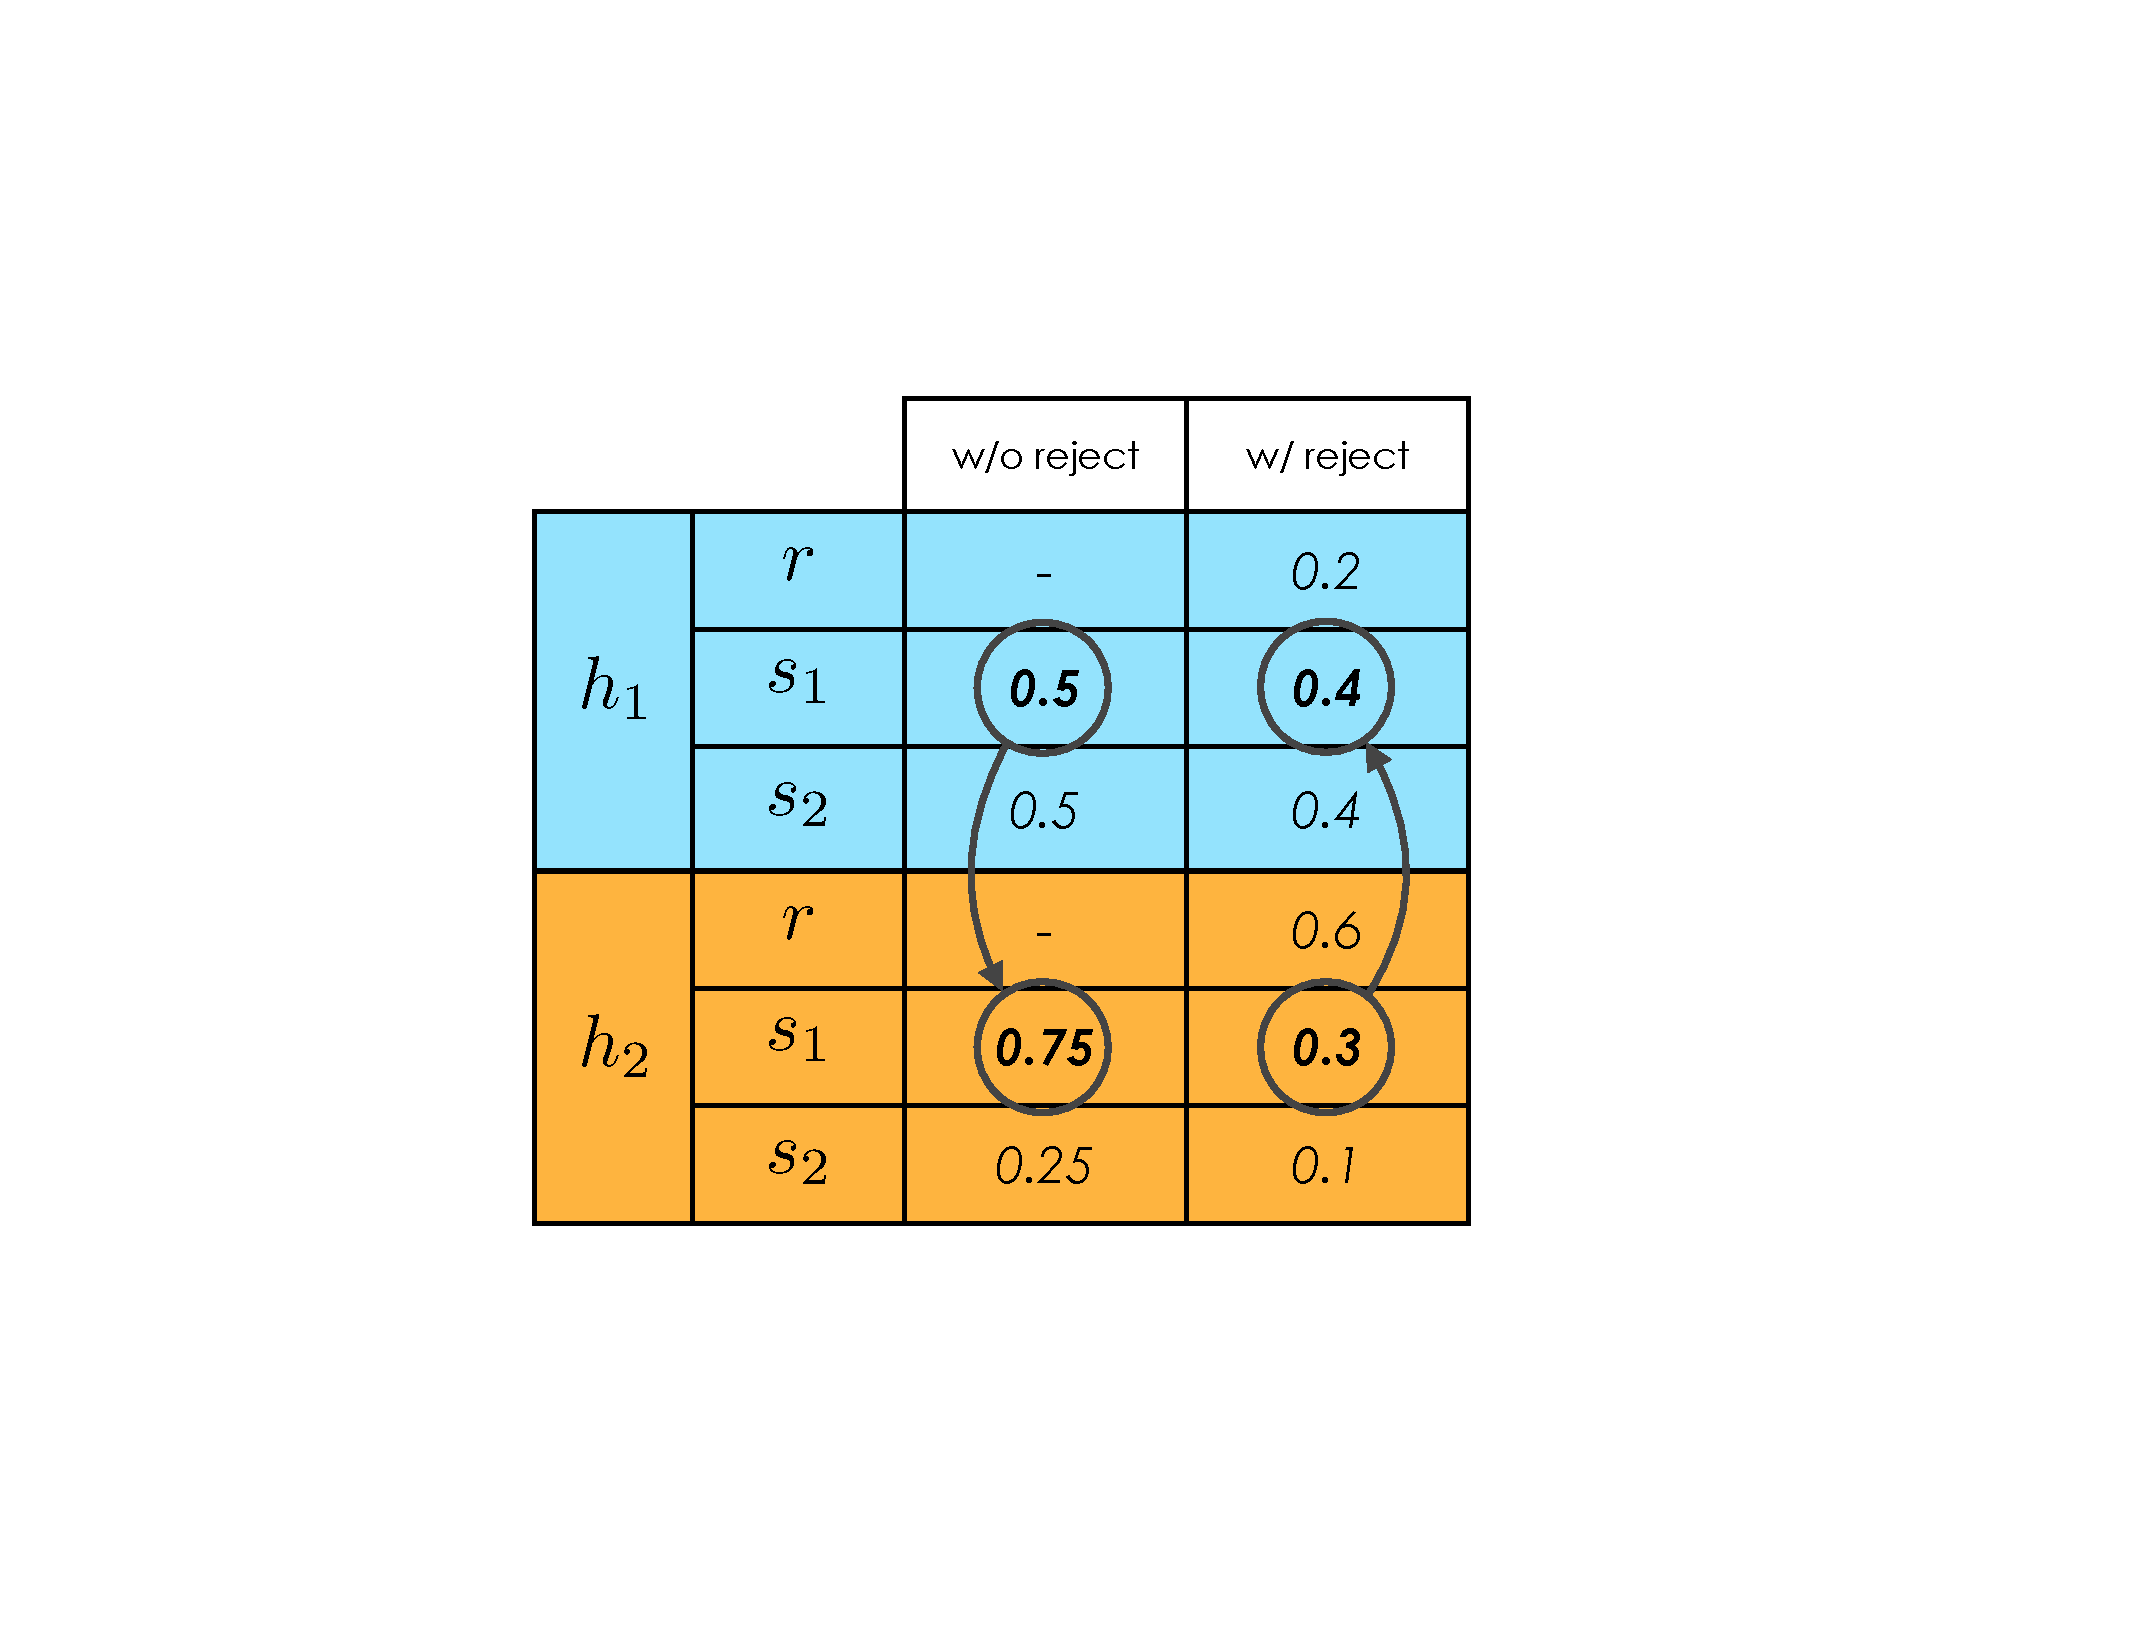
\includegraphics[width=0.6\linewidth]{figures/reject_vs_no_reject.pdf}
\caption{
Example of a case where modeling the reject option results in vastly different recommendation behavior.
Consider surfer $s_1$'s perspective: without modeling the reject option, $h_2$ looks more likely to accept $s_1$.
When modeling the reject option, however, the probabilities change and $h_1$ is now more likely to accept $s_1$, due to the ability to model how picky $h_2$ actually is.}
\label{fig:reject_vs_no_reject}
\end{figure}

We predict the probability that a host $h$ chooses the surfers $s_{k^*}$ among a competitorset $S=\{ s_1, \dots, s_n\}$ or that he rejects all of them using the following logistic model:
\begin{eqnarray}
p(s_k | h, S) &=& \frac{\exp(\theta^T \Phi(s_k,h))}{\sum_{s_j \in S} \exp(\theta^T \Phi(s_j,h)) + \exp(r)} \\
p(\text{reject} | h, S) &=& \frac{\exp(r)}{\sum_{s_j \in S} \exp(\theta^T \Phi(s_j,h)) + \exp(r)}
\end{eqnarray}
In this formulation, each surfer $s_k$ receives a score $\exp(\theta^T \Phi(s_k,h))$ modeling the natural competition between multiple surfers that requested to stay with the host. In the end, we predict that the surfer with the highest score wins, or that everybody gets rejected if the rejectscore $\exp{(r)}$ is largest. 
Further, we implicitly learn a bias term by appending a one to the feature representation $\Phi(s_k,h)$.
Note, however, that this is not exactly the standard multinomial logistic regression model since in our case we have the same parameters but we have different features for the different ``classes'' (i.e. surfers).

Even though we essentially just rank the candidates for the host that sent a couchrequest it is still important to model the possibility of rejection. It enables us to model actual probabilities that are very important from the perspective of the surfers. For them, we rank the different host in order of the likelihood that their couchrequest to these hosts would be successful. Because we compare different hosts to each other here their pickiness actually matters to the surfer. See Figure \ref{fig:reject_vs_no_reject} for an example where modeling 

The parameters (to be learned) for this model capture what hosts prefer in surfers and their request, i.e. their language, nationality, age, gender etc. Because the feature $\Phi(s_k,h)$ depends on both the surfer and the host we also model that i.e. Americans like to host surfers from certain countries and that hosts generally prefer to have a language in common with the couchsurfer.

These preferences might be very different from host to host though. Also, some hosts might be more picky than others rejecting almost all requests and we should be able to capure that, too. Therefore, we introduce host-specific parameters $\theta_h$ and $r_h$ to model these effects. Because we have millions of hosts storing all these parameters explicitly would require tens of gigabytes of memory. % TODO should the hashing trick get it's own section? I would say explain it a bit in related work and a bit here again
Since this is infeasible we make use of the hashing trick to hash the parameters into an array of predefined size (allowing for collisions between parameters). Thereby, we can control how much memory we want to allocate for personalization. This trick has been successfully applied e.g. for spam classification \cite{Attenberg2009}.
Including personalized parameters leads to the following updated model:
\begin{eqnarray}
p(s_k | h, S) &=& \frac{\exp((\theta + \theta_h)^T \Phi(s_k,h))}{\sum_{s_j \in S} \exp((\theta + \theta_h)^T \Phi(s_j,h)) + \exp(r + r_{h})} \\
p(\text{reject} | h, S) &=& \frac{\exp(r+r_{h})}{\sum_{s_j \in S} \exp((\theta + \theta_h)^T \Phi(s_j,h)) + \exp(r + r_{h})}
\end{eqnarray}
As an error measure we use the negative log-likelihood of the data with $l_2$-penalty on the parameters for regularization. In our Stochastic Gradient Descent (SGD), we randomly sample a host $h$ and a competitorset $S=\{ s_1, \dots, s_n\}$. There are two cases: either there is one surfer $s_{k^*}$ that got accepted, or everybody got rejected. We obtain the following update equations for SGD where $\lambda_1, \lambda_2$ are regularization parameters and $\eta$ is the learning rate

1. Case: Some surfer $s_{k^*}$ gets chosen (no reject):
\begin{eqnarray}
\theta &\leftarrow& (1- \eta \lambda_1) \theta - \eta (\sum_{j \in S_n} p(s_j | h, S) \Phi(s_j,h_n) - \Phi(s_{k^*},h_n))\\
r &\leftarrow& (1- \eta \lambda_2) r - \eta p(\text{reject} | h_n, S_n)
\end{eqnarray}

2. Case: No surfer gets chosen (reject):
\begin{eqnarray}
\theta &\leftarrow& (1- \eta \lambda_1) \theta - \eta (\sum_{j \in S_n} p(s_k | h, S) \Phi(s_j,h_n))\\
r &\leftarrow& (1- \eta \lambda_2) r - \eta (p(\text{reject} | h_n, S_n)-1)
\end{eqnarray}

The update equations for $\theta_h$ and $r_h$ are the same as the ones for $\theta$ and $r$, respectively, but they are only updated for the current host $h$. 
Also note that these update equations intuitively make sense . For $\theta$ we essentially increase the contribution from the features of the winner and decrease it for all the losers always according to their probability of being chosen. This means that if the model did a bad prediction we update our parameters more than normally. For $r$ it is similar in the sense that we increase it whenever everybody actually got rejected and decrease it if we had a winner.


%%%%%%%%%%%%%%%%%%%%%%%%%%%
% this is where the old stuff starts
%-----------------OLD STUFF------
%
%\begin{eqnarray}
%p(s_k | h_n, S_n) &=& \frac{\exp(\theta^T \Phi(s_k,h_n))}{\sum_{j \in S_n} \exp(\theta^T \Phi(s_j,h_n)) + \exp(r + r_{h_n})} \\
%p(\text{reject} | h_n, S_n) &=& \frac{\exp(r+r_{h_n})}{\sum_{j \in S_n} \exp(\theta^T \Phi(s_j,h_n)) + \exp(r + r_{h_n})}
%\end{eqnarray}
%Note that $\Phi(s_k,h_n)$ also implicitly depends on the couchrequest (e.g. date, whether the host is already booked, etc.).
%
%To have hostspecific parameters we would replace $\theta$ by $\theta + \theta_h$. 
%
%Further, we want to add regularization for $\theta, \theta_h, r_{h_n}$.
%
%Error (negative log likelihood)
%\begin{eqnarray}
%E(\theta, r, r_{h_n}) &=& - \log p(\{s_k\} | \{h_n\}, \{S_n\})\\
%&=& - \log [ \prod_{n=1}^N \prod_{k=1}^K p(s_k | h_n, S_n)^{t_{nk}}]\\
%&=&  - \sum_{n=1}^N \sum_{k=1}^K t_{nk} \log p(s_k | h_n, S_n)
%\end{eqnarray}
%
%To derive the gradient descent update steps we will take derivatives of $E(\theta, r, r_{h_n})$ wrt. $\theta, r, r_{h_n}$. Because we will do stochastic gradient descent we will basically ignore the sum over $n$ in the end (over different ``competitor sets $S_n$'') and just choose one at random. Note that here, we can just sample uniformly from all sets or sample a host first, and given that host, sample on of his sets. The latter will achieve that all hosts have the sample influence on the learning but we will have to discuss/test whether we actually want that.
%
%We generally have:
%\begin{eqnarray}
%\frac{d}{d \theta} E(\theta, r, r_{h_n}) &=& - \sum_{n=1}^N \sum_{k=1}^K t_{nk} \frac{d}{d \theta}  \log p(s_k | h_n, S_n) \\
%&=& - \sum_{n=1}^N \sum_{k=1}^K t_{nk} \frac{1}{p(s_k | h_n, S_n)} \frac{d}{d \theta} p(s_k | h_n, S_n)
%\end{eqnarray}
%
%Now we look at the individual derivatives of $p(s_k | h_n, S_n)$ and $p(\text{reject} | h_n, S_n)$.
%
%1. Case: Some surfer $s_k$ gets chosen (no reject):
%\begin{eqnarray}
%\frac{d}{d \theta} p(s_k | h_n, S_n) = \frac{d}{d \theta} \frac{\exp(\theta^T \Phi(s_k,h_n))}{\sum_{j \in S_n} \exp(\theta^T \Phi(s_j,h_n)) + \exp(r + r_{h_n})} \\
%= \frac{\Phi(s_k,h_n) [\sum_{j \in S_n} \exp(\theta^T \Phi(s_j,h_n)) + \exp(r + r_{h_n})]}{\sum_{j \in S_n} \exp(\theta^T \Phi(s_j,h_n)) + \exp(r + r_{h_n})} \\
%- \frac{\exp(\theta^T \Phi(s_k,h_n)) [\sum_{j \in S_n} \Phi(s_j,h_n) \exp(\theta^T \Phi(s_j,h_n))]}{\sum_{j \in S_n} \exp(\theta^T \Phi(s_j,h_n)) + \exp(r + r_{h_n})}\\
%= \Phi(s_k,h_n) p(s_k | h_n, S_n) - p(s_k | h_n, S_n) \frac{\sum_{j \in S_n} \Phi(s_j,h_n) \exp(\theta^T \Phi(s_j,h_n))}{\sum_{j \in S_n} \exp(\theta^T \Phi(s_j,h_n)) + \exp(r + r_{h_n})}\\
%= p(s_k | h_n, S_n) (\Phi(s_k,h_n) - \sum_{j \in S_n} w_{jn} \Phi(s_j,h_n))
%\end{eqnarray}
%where $w_{jn}=\frac{\exp(\theta^T \Phi(s_j,h_n))}{\sum_{j \in S_n} \exp(\theta^T \Phi(s_j,h_n)) + \exp(r + r_{h_n})}$.
%
%Thus, we get:
%\begin{eqnarray}
%\frac{d}{d \theta} E(\theta, r, r_{h_n}) = - \sum_{n=1}^N \sum_{k=1}^K t_{nk} \frac{1}{p(s_k | h_n, S_n)} \frac{d}{d \theta} p(s_k | h_n, S_n)\\
%= - \sum_{n=1}^N \sum_{k=1}^K t_{nk} (\Phi(s_k,h_n) - \sum_{j \in S_n} w_{jn} \Phi(s_j,h_n)) \\
%= \sum_{n=1}^N (\sum_{j \in S_n} w_{jn} \Phi(s_j,h_n) - \Phi(s_{k^*},h_n))
%\end{eqnarray}
%where $s_{k^*}$ is the surfer that got accepted from the competitor set $S_n$.
%
%Similarly, taking the derivative wrt. $r$ ($r_{h_n}$ should be exactly the same) we obtain:
%\begin{eqnarray}
%\frac{d}{d r} p(s_k | h_n, S_n) = -  p(s_k | h_n, S_n)  \frac{\exp(r + r_{h_n})}{\sum_{j \in S_n} \exp(\theta^T \Phi(s_j,h_n)) + \exp(r + r_{h_n})}
%\end{eqnarray}
%Thus, we get:
%\begin{eqnarray}
%\frac{d}{d r} E(\theta, r, r_{h_n}) = - \sum_{n=1}^N \sum_{k=1}^K t_{nk} \frac{1}{p(s_k | h_n, S_n)} \frac{d}{d r} p(s_k | h_n, S_n)\\
%= \sum_{n=1}^N \sum_{k=1}^K t_{nk} \frac{\exp(r + r_{h_n})}{\sum_{j \in S_n} \exp(\theta^T \Phi(s_j,h_n)) + \exp(r + r_{h_n})} \\
%= \sum_{n=1}^N \frac{\exp(r + r_{h_n})}{\sum_{j \in S_n} \exp(\theta^T \Phi(s_j,h_n)) + \exp(r + r_{h_n})}
%\end{eqnarray}
%
%
%
%2. Case: No surfer gets chosen (reject):
%\begin{eqnarray}
%\frac{d}{d \theta} p(\text{reject} | h_n, S_n) = \frac{d}{d \theta} \frac{\exp(r+r_{h_n})}{\sum_{j \in S_n} \exp(\theta^T \Phi(s_j,h_n)) + \exp(r + r_{h_n})}\\
%= - p(\text{reject} | h_n, S_n) \frac{\sum_{j \in S_n} \Phi(s_j,h_n) \exp(\theta^T \Phi(s_j,h_n))}{\sum_{j \in S_n} \exp(\theta^T \Phi(s_j,h_n)) + \exp(r + r_{h_n})} \\
%= - p(\text{reject} | h_n, S_n) \sum_{j \in S_n} w_{jn} \Phi(s_j,h_n)
%\end{eqnarray}
%Thus, we get:
%\begin{eqnarray}
%\frac{d}{d \theta} E(\theta, r, r_{h_n}) = - \sum_{n=1}^N \sum_{k=1}^K t_{nk} \frac{1}{p(\text{reject} | h_n, S_n)} \frac{d}{d \theta} p(\text{reject} | h_n, S_n)\\
%= \sum_{n=1}^N (\sum_{j \in S_n} w_{jn} \Phi(s_j,h_n))
%\end{eqnarray}
%
%
%
%Again, taking the derivative wrt. $r$ ($r_{h_n}$ should be exactly the same) we obtain:
%\begin{eqnarray}
%\frac{d}{d r} p(\text{reject} | h_n, S_n) = p(\text{reject} | h_n, S_n) - p(\text{reject} | h_n, S_n)^2\\
%= p(\text{reject} | h_n, S_n) (1 - p(\text{reject} | h_n, S_n))\\
%\end{eqnarray}
%Thus, we get:
%\begin{eqnarray}
%\frac{d}{d r} E(\theta, r, r_{h_n}) = - \sum_{n=1}^N \sum_{k=1}^K t_{nk} \frac{1}{p(\text{reject} | h_n, S_n)} \frac{d}{d \theta} p(\text{reject} | h_n, S_n)\\
%= \sum_{n=1}^N (p(\text{reject} | h_n, S_n)-1)
%\end{eqnarray}
%
%
%\paragraph{The final update equations}
%
%Finally, for stochastic gradient descent the following update equations hold. We simply sample a host $h_n$ and competitor set $S_n$. Note that the following equations do not contain regularization, yet (although trivial).
%
%1. Case: Some surfer $s_{k^*}$ gets chosen (no reject):
%\begin{eqnarray}
%\theta \leftarrow \theta - \eta (\sum_{j \in S_n} w_{jn} \Phi(s_j,h_n) - \Phi(s_{k^*},h_n))\\
%r \leftarrow r - \eta \frac{\exp(r + r_{h_n})}{\sum_{j \in S_n} \exp(\theta^T \Phi(s_j,h_n)) + \exp(r + r_{h_n})}
%\end{eqnarray}
%where, again, $w_{jn}=\frac{\exp(\theta^T \Phi(s_j,h_n))}{\sum_{j \in S_n} \exp(\theta^T \Phi(s_j,h_n)) + \exp(r + r_{h_n})}$.
%
%2. Case: No surfer gets chosen (reject):
%\begin{eqnarray}
%\theta \leftarrow \theta - \eta (\sum_{j \in S_n} w_{jn} \Phi(s_j,h_n))\\
%r \leftarrow r - \eta (p(\text{reject} | h_n, S_n)-1)
%\end{eqnarray}
%
%For $l_2$-regularization, e.g. of $\theta$, just add $- \eta \lambda \theta$ to the update equation.
%

% !TEX root=report.tex
\section{Evaluation} \label{sec:evaluation}

The CouchSurfing dataset was made available to the authors in the form of an anonymized MySQL database dump.
As shown in \autoref{fig:requests_distribution}, the distribution of number of requests received is roughly logarithmic on a logarithmic scale.

\begin{figure}[ht]
\centering
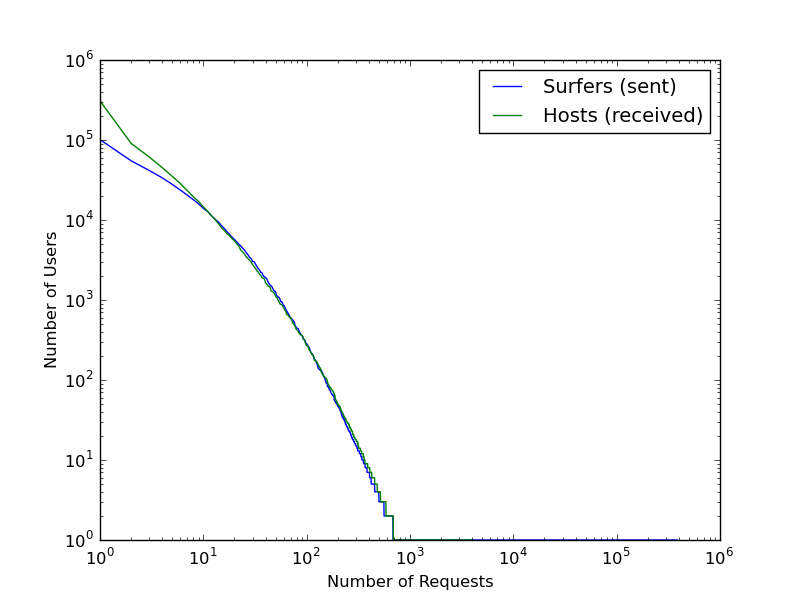
\includegraphics[width=1\linewidth]{figures/req_received_dist2.png}
\caption{Distribution of requests received by a host. \todo{Tobi: these numbers must be incorrect}}
\label{fig:requests_distribution}
\end{figure}

\todo{summary of statistics about the data, nr surfers/hosts/couchrequests, nr competitorsets, distribution over size of competitorsets}

\todo{Evaluation measures: prediction accuracy, mean normalized rank of winner}

\todo{Baselines: [so far we have some code for random baseline + allreject baseline but nothing more fancy, also CS hasn't responded to our email]}

\todo{Results (In progress.)}


\bibliographystyle{ieeetr}
\small
\bibliography{sergeyk_csrec}
\end{document}
